\graphicspath{{images/}} % Location of the slide background and figure files

%----------------------------------------------------------------------------------------
%	TITLE PAGE
%----------------------------------------------------------------------------------------

\title[Stress regulation]{Stress Regulation} % The short title appears at the bottom of every slide, the full title is only on the title page
\subtitle{What is Stress and What can We do about It?}
\mode<all>

\author{Raphael Nussbaum} % Your name
\institute[Stress Regulation] % Your institution as it will appear on the bottom of every slide, may be shorthand to save space
{
AJ Tutoring Nerd Fest \\
%Stress regulation YouTube channel \\ % Your institution for the title page
\medskip
\textit{raphaelnussbaum@ajtutoring.com}
%regulate.stress@gmail.com} % Your email address
}
\date{\today} % Date, can be changed to a custom date


\mode*

\mode<all>
\begin{document}
\mode*

\mode
<presentation>
{ \begin{frame}
\titlepage % Print the title page as the first slide
\end{frame}}

\maketitle

%\begin{frame}
%\frametitle{Overview} % Table of contents slide, comment this block out to remove it
%\tableofcontents % Throughout your presentation, if you choose to use \subsection{} and \subsubsection{} commands, these will automatically be printed on this slide as an overview of your presentation
%\end{frame}

%----------------------------------------------------------------------------------------
%	PRESENTATION SLIDES
%----------------------------------------------------------------------------------------

%------------------------------------------------
\section{Goals} 
 % Sections can be created in order to organize your presentation into discrete blocks, all sections and subsections are automatically printed in the table of contents as an overview of the talk
%------------------------------------------------

%\subsection{Subsection Example} % A subsection can be created just before a set of slides with a common theme to further break down your presentation into chunks

% \mode<all>
% \begin{frame}
\frametitle{What can be done?}
\begin{columns}[c] % The "c" option specifies centered vertical alignment while the "t" option is used for top vertical alignment
\column{.3\textwidth} % Left column and width

\includegraphics[width=\linewidth]{Question.png}
\column{0.7\textwidth} % Right column and width

\begin{itemize}
\item \structure{regulate}
\item \structure{negative stress} vs \structure{positive stress}
\item \structure{stress resistance} 
\item \structure{relaxation} and \structure{mindfulness} exercises
\item \structure{Eat consciously}
\item A \structure{mindful life} 
\end{itemize}
\end{columns}
\end{frame}

 % okay for article
% \mode*

% %------------------------------------------------
% \section{Theory}
% \subsection{Stress}
% \subsubsection{What is Stress?}

% \mode<all>
% \documentclass[../main.tex]{subfiles}
\graphicspath{{\subfix{../images/}}}
\begin{document}


\index{stress!definition}
The formal definition of Stress is the attempt of the body to get back to equilibrium (homeostasis)\index{homeostasis} as fast as possible after an irritating stimulus.
There's a distinction to be made between negative stress which get caused by ``seeming impossible''
 situations and positive stress caused in situations which are subjectively perceived as surmountable.
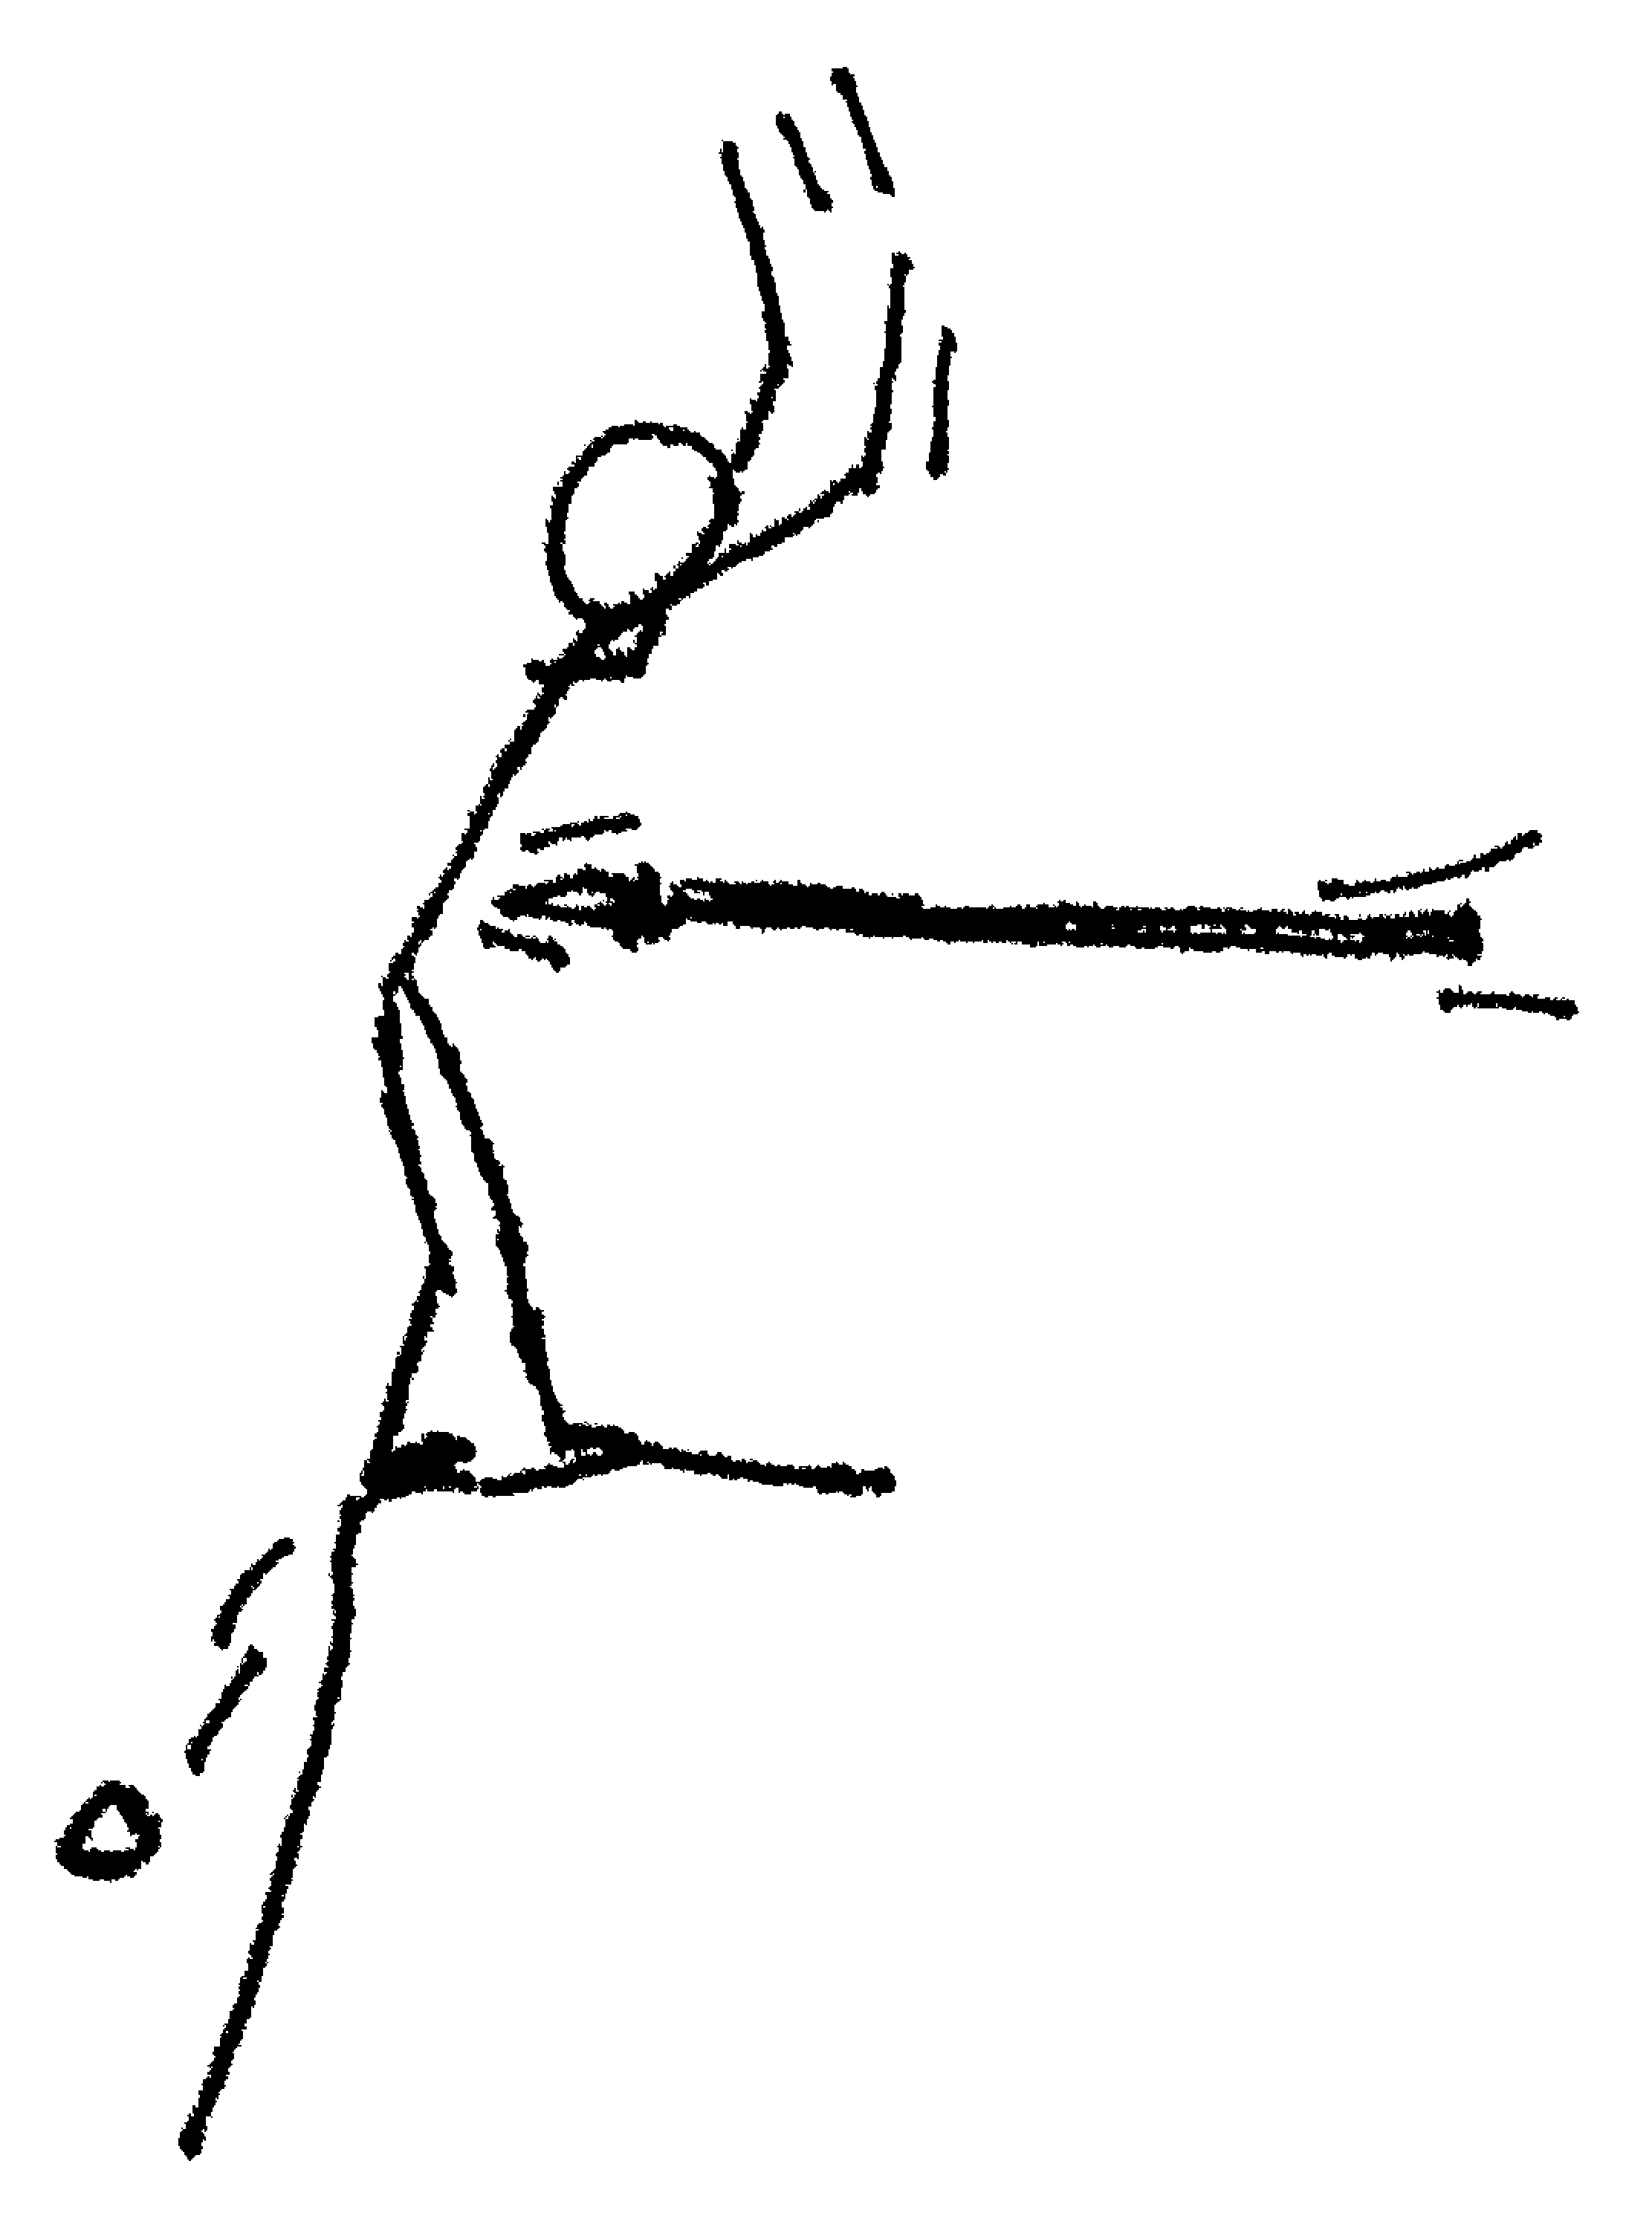
\includegraphics[width=3cm]{Guy-Edge}\label{sf:edge}

Humans can't live without stress, for many situations it needs a heightened action potential. For instance stress releases the stress hormones in the body. They trigger diverse reactions in the body: the hearth rate increases, brain and lungs get better supplied and the senses get sharpened.

The term stress\index{stress!definition} was introduced 1936 by the Austrian-Canadian doctor Hans Selye\index{Selye, Hans} to describe the \emph{reaction of biological systems to pressure}. The term was meant to neutrally describe what happens in the body in such situations.
It's important to note, that it didn't have the negative connotation yet, that nowadays is often attributed to the term but in it's original meaning it should neutrally describe what happens to the body when it is under pressure.

\subsubsection{Is Stress Needed?}

This question is less harmless than it looks like. First of all, we have to distinguish between two types of stress:
	\begin{description}
		\item[Negative Stress]\index{stress!negative} triggered by ``seemingly impossible situations''
		\item[Positive Stress]\index{stress!positive} triggered in situations which are subjectively perceived as manageable
	\end{description}
	
Humans couldn't possibly live without stress. Stress is a necessary ingredient for a human's ability to thrive and grow on obstacles. It produces an heightened action potential, which is needed in many situations.

Nowadays, the expression stress is the general term for the mental and bodily reactions to inner or outer impulses, which humans perceive as pleasant or as burdening.
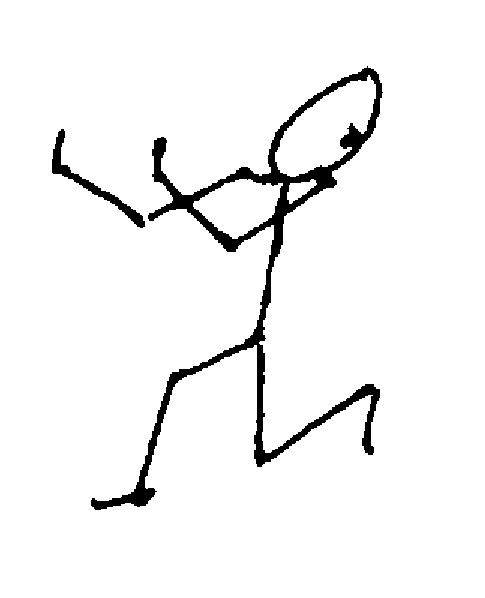
\includegraphics[width=2cm]{Guy_Distress}
\hspace{5cm}
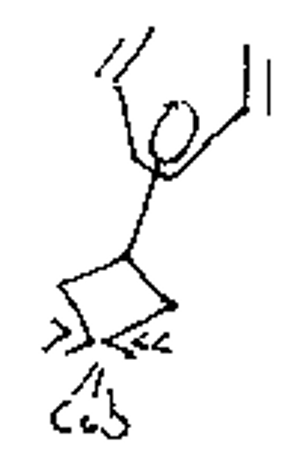
\includegraphics[width=2cm]{Guy_Eustress}\label{sf:eustress}

\section{Eustress vs. Distress}

\emph{Eu--stress}\index{Eustress (Eu--stress)} (Greek ``Eu'' = ``good'') is exciting stress and vital for humans. 
Eustress is a situation, which we perceive as increasing our well--being. 

On the other hand, \emph{Dis--stress}\index{Distress (Dis--stress)} (Greek ``dis'' = ``against'') is life endangering stress. In this situation we feel a burden or pressure from inside or outside.



\epigraph{Life isn't about waiting for the storm to pass \ldots  \\ 
It's about learning to dance in the rain.}{\textit{Anonymous}, more recently attributed to \textit{Vivian Greene}}


\subsubsection{Conclusion}
\noindent In light of the distinctions we made, let's talk about the best stress regulation measure\index{stress!regulation} possible:
\begin{itemize}
\item Distress (Dis--stress) can be changed to eustress with appropriate methods, taking into account the individual tenacity and sensitivities.
\item As soon as we realize that we decide ourselves about the perception of pleasurable stress (eustress) and painful stress (distress) we get our freedom back. 
\item The taxing stress has to be let go on a conscious level. Many people think they are in stress but aren't, and the other way round.
\end{itemize}

\epigraph{Human: learn to dance, so when you get to heaven the angels know what to do with you.}{\textit{St. Augustine}}


%------------------------------------------------
\end{document} %Good
% \mode*

% \subsection{Medical Background}
% \subsubsection{What happens in the Body?}

% \mode<all>
% \documentclass[../Book.Stress_regulation.tex]{subfiles}
\graphicspath{{\subfix{../images/}}}
\begin{document}

\epigraph{Pleasure in the job puts perfection in the work.}{\textit{Aristotle}}

\subsubsection{Stress Hormones}


During stress, the so called stress hormones\index{stress hormones} get released in our body: \emph{noradrenaline} and \emph{adrenaline}.
Their job is to provide as much {energy} in the from of sugar from the liver to the body, as fast as possible.
The fastest acting one is noradrenaline\index{stress hormones!noradrenaline}, which readies our body for the incoming stressful situation.


% ------------------------------------------------


\subsubsection{Noradrenaline vs. Adrenaline}

\begin{figure}[htb]
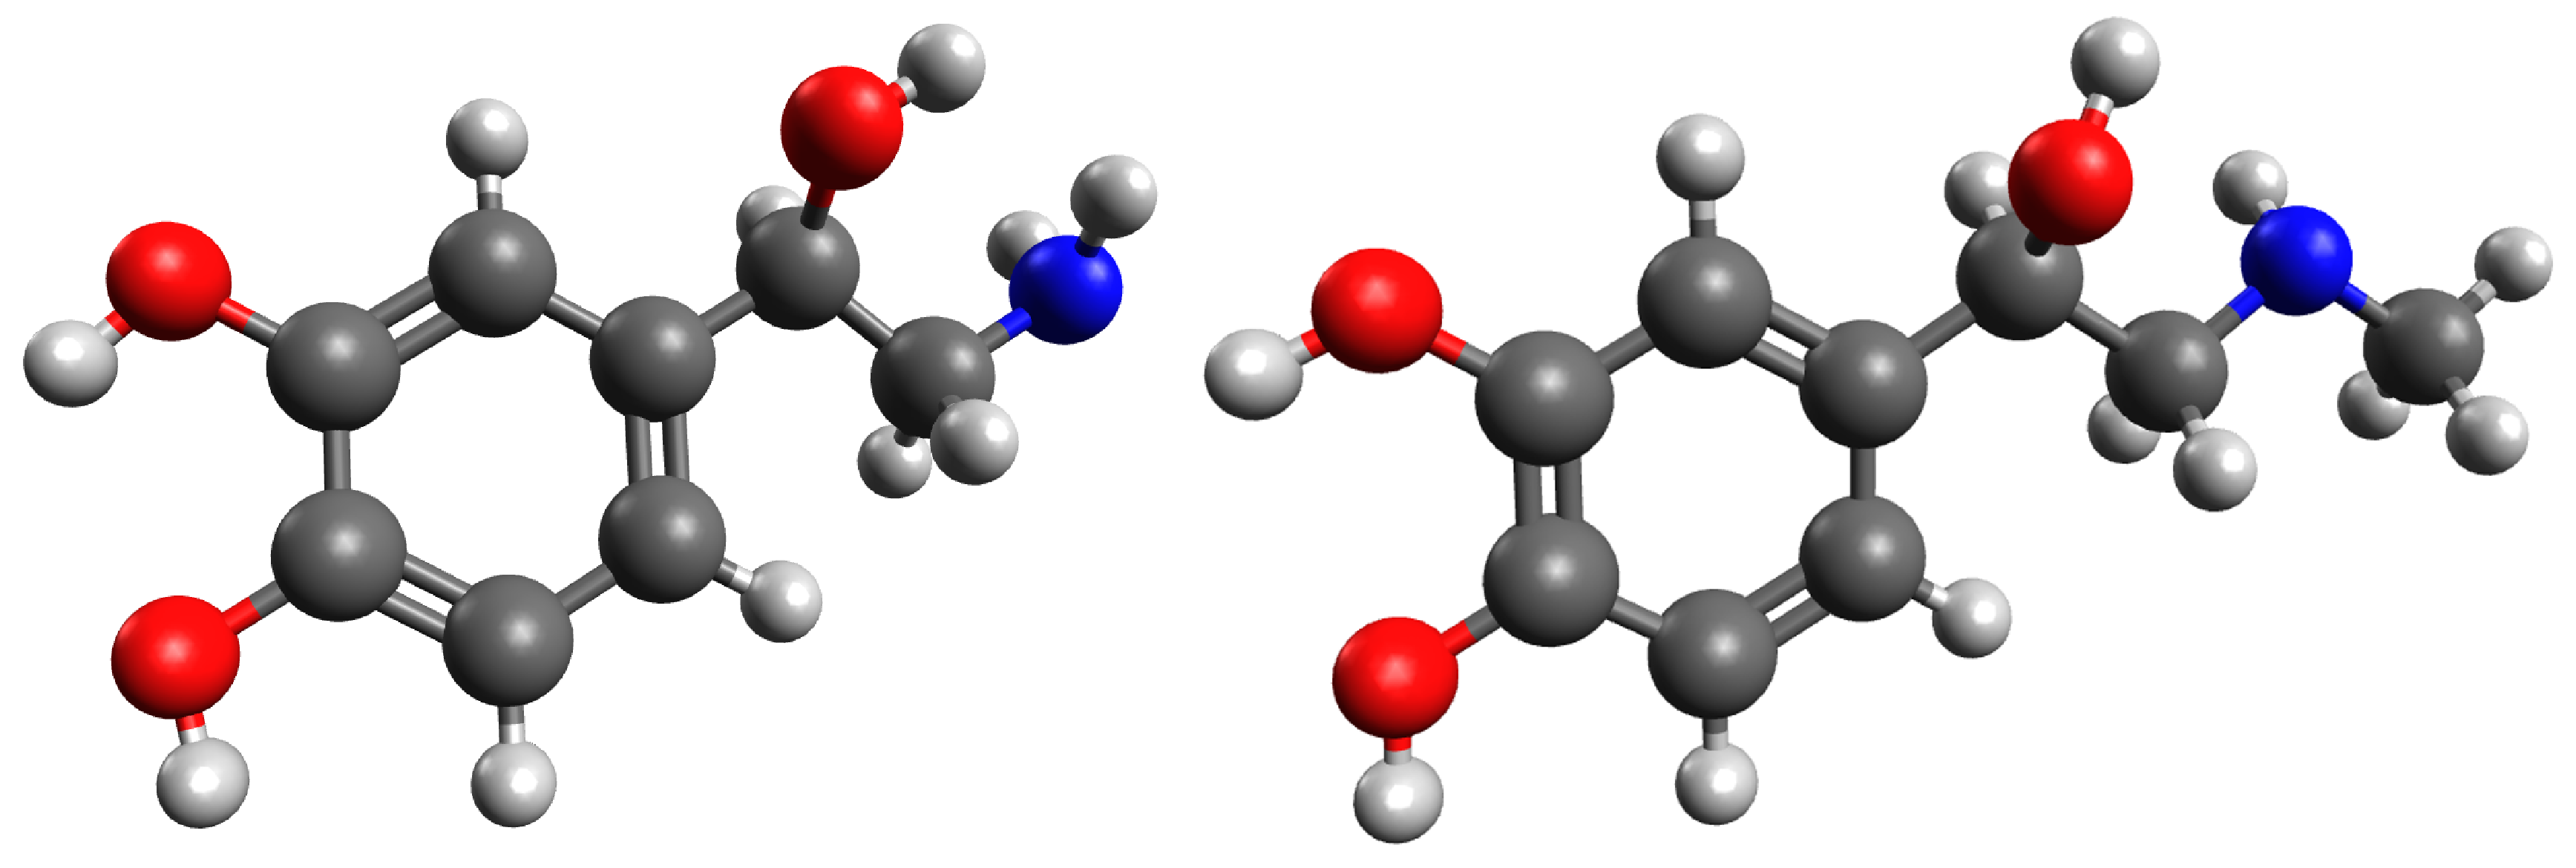
\includegraphics[width=12cm]{Nor_Adrenaline}
\caption{The structures of noradrenaline and adrenaline}
\end{figure}

Noradrenaline has it's {own release system} in the body. It gets released by free nerve endings of the somatic nervous system\index{nervous system!somatic}.
The somatic nerves are the nerves situated in our body as opposed to the ones in the central nervous system.
It bypasses the slower blood stream transport system.
Noradrenaline prepares us in a {``cool'' way} for danger, by providing muscles instantaneously with energy in the form of glucose (sugar).
The actions of noradrenaline doesn't get noticed by the hearth, so the hearth rate doesn't get affected yet.
Both, eustress and distress cause the release of catecholamines\footnote{Catecholamines is a medical expression, most often used in it's plural form, catecholamines. Another name is brenzcatechineamines. They are a class of body's own and synthetic chemical compounds, which have a stimulating effect at the sympathetic alpha and beta receptors of the hearth--circulation. Therefore catecholamines are sympathomimetics. They all have a similar structure and are related to phenylethylamines and substances related to adrenaline.}, noradrenaline (over the somatic nervous system\footnote{The nervous system of the body, as opposed to the central nervous system.}) and adrenaline (over the bloodstream) get released.



\subsubsection{The Typical Stress Reaction}
The ``typical'' stress reaction doesn't exist, it's a \emph{process}: the body tries to get back into {equilibrium} after an irritating stimulus, which can be perceived as positive or negative.
The emotions going along with this aren't uniform.
They depend on the {personality structure}\index{personality!structure} and the {intensity} of the of the experiencing.

But what is for sure is that every burden which hits us and which we don't {consciously acknowledge} will express itself sooner or later by the means of the body.

\end{document}

 %Good
% \mode*

% %------------------------------------------------
% \subsection{Coping}
% \mode<all>
% \documentclass[../Book.Stress_regulation.tex]{subfiles}
\graphicspath{{\subfix{../images/}}}
\begin{document}



%\subsubsection{Anticipatory Coping}

\epigraph{Giving up smoking is the easiest thing in the world. I know, because I've done it thousands of times.}{\textit{Mark Twain}}

Anticipatory coping\footnote{cope, to overcome --- anticipate, is to consider an upcoming event}\index{coping!anticipatory} is efforts done {in advance} of a possible stress,  with the goal to {overcome}, reduce or tolerate the {imbalance between perceived requirements and available resources}.

Two types of coping strategies can be distinguished.

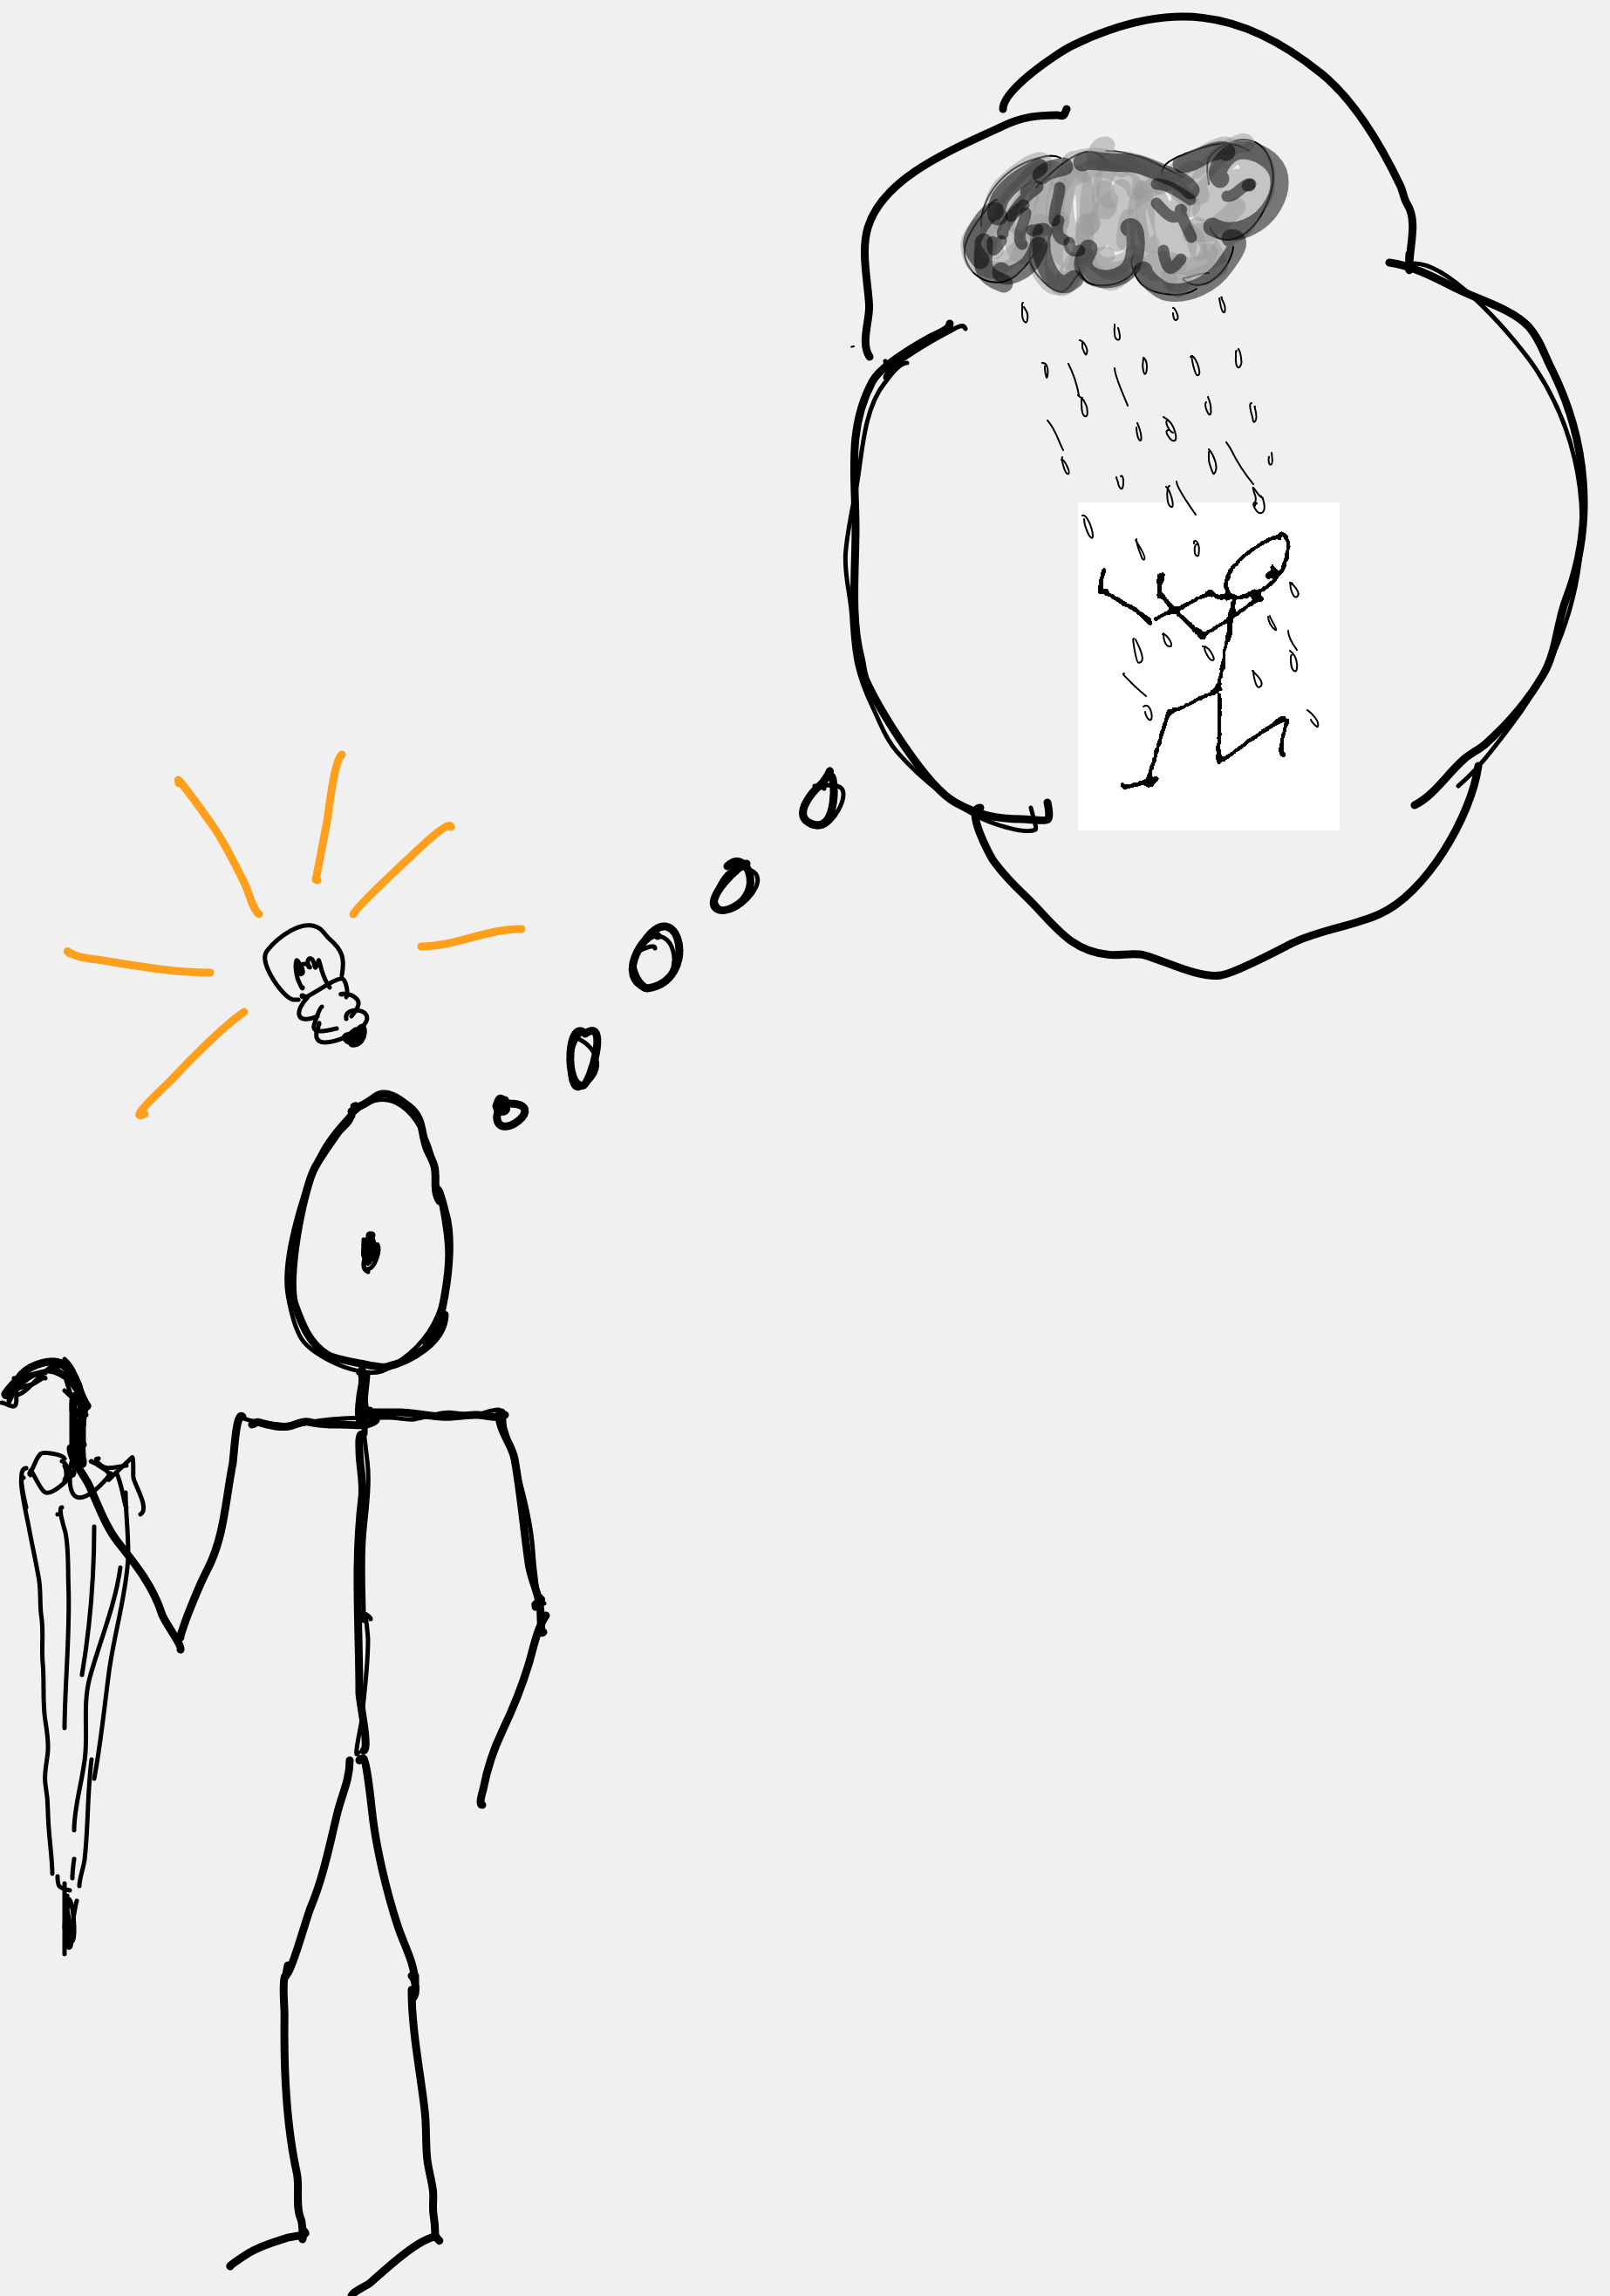
\includegraphics[width=4cm]{ACoping}\label{sf:coping}

 \begin{description}
\item[Problem Oriented Coping]\index{coping!problem oriented} attempts to change the stressor or the relation to it by the means of {direct actions} and/or problem solving activities, such as to fight, in order to destroy, neutralize or weaken the threat. Flight in order to remove yourself from the threat is another possible action, or then looking for possibilities for fight or flight, like to lie, to negotiate or to make a compromise. Yet another way is to avoid future stress, by behaving in a way to increase the own tolerance or to decrease the expected future stress.
\item[Emotion Oriented Coping]\index{coping!emotion oriented} is an attempt to change yourself with activities, which make you {feel better}, without changing the stressor.
\end{description}

Some examples are relaxation and Bio feedback as Body centered activities, mind centered activities could be planning distractions, day dreaming or thinking about yourself or then therapy to regulate the conscious and subconscious mechanism which leads to additional fear.



\end{document} %Good
% \mode*

% %-------------------------------------------------
% \subsection{General adaptation system GAS}

% \mode<all>
% \documentclass[../Book.Stress_regulation.tex]{subfiles}
\graphicspath{{\subfix{../images/}}}
\begin{document}


Stress is the attempt of the body, to {adapt} to different types of pressure. 
 In science, this process is called the {General Adaptation System} GAS\index{system!general adaptation system GAS}.
 {Long--lasting massive stress} situations induce in the organism three distinct phases.

 \epigraph{It is only with the hearth that one can see right, what is essential is invisible to the eye.}{\textit{Antoine de Saint-Exup\'ery}}
 
 \begin{enumerate}
 \item The \emph{Alarm reaction}\index{reaction!alarm reaction} is the first phase.
   It puts the body in a state of shock\index{shock} directly after the stressor effect registers.
   A lot of {physiological parameters regulate down eventually fail}. These are a lot of small units, which co--create and define the processes of life.
Soon after, the body starts the {counter--regulation}\index{regulation!counter regulation}, in order to be able maintain the body--mind system's integrity. The vegetative nervous system tries to counteract and balance the two effects.
\item The \emph{Resistance Phase} is triggered by {repeated stress} influence or by {ongoing} influence
The body then activates all available means to overcome the stress reaction. This is called the \emph{psycho physiological adaptation}.\index{adaptation!psycho physiological}
\item In the Exhaustion Phase the organism {decompensates}.\index{decompensation}
The {regulation functions} which have been build up by the body during the alarm reaction disappear and the {adaptation} to the stress situation {crashes}.
In the meanwhile the {immune functions} get down regulated and {organic impairments} occur.
 \end{enumerate}
\end{document}
%Good
% \mode*

% \subsection{Limbic System} 
% \mode<all>
% \documentclass[../Book.Stress_regulation.tex]{subfiles}
\graphicspath{{\subfix{../images/}}}
\begin{document}


\subsubsection{The Start of the Stress Reaction  ---  Seat of the Alarm Central}
Stress starts with the {sensory organs}. Endogenous\footnote{Coming from the inside} and exogenous\footnote{Coming from the outside} {sensory impulses} get registered at the receptor of the {sensory cells}.
 The sensory impulses creates an {electric impulse} in the nervous cells which transmit the information, which is called an {excitation}.
 The impressions get passed on to the {limbic system}, which {processes them} before they get transmitted to the brain.


\begin{figure}[htb]
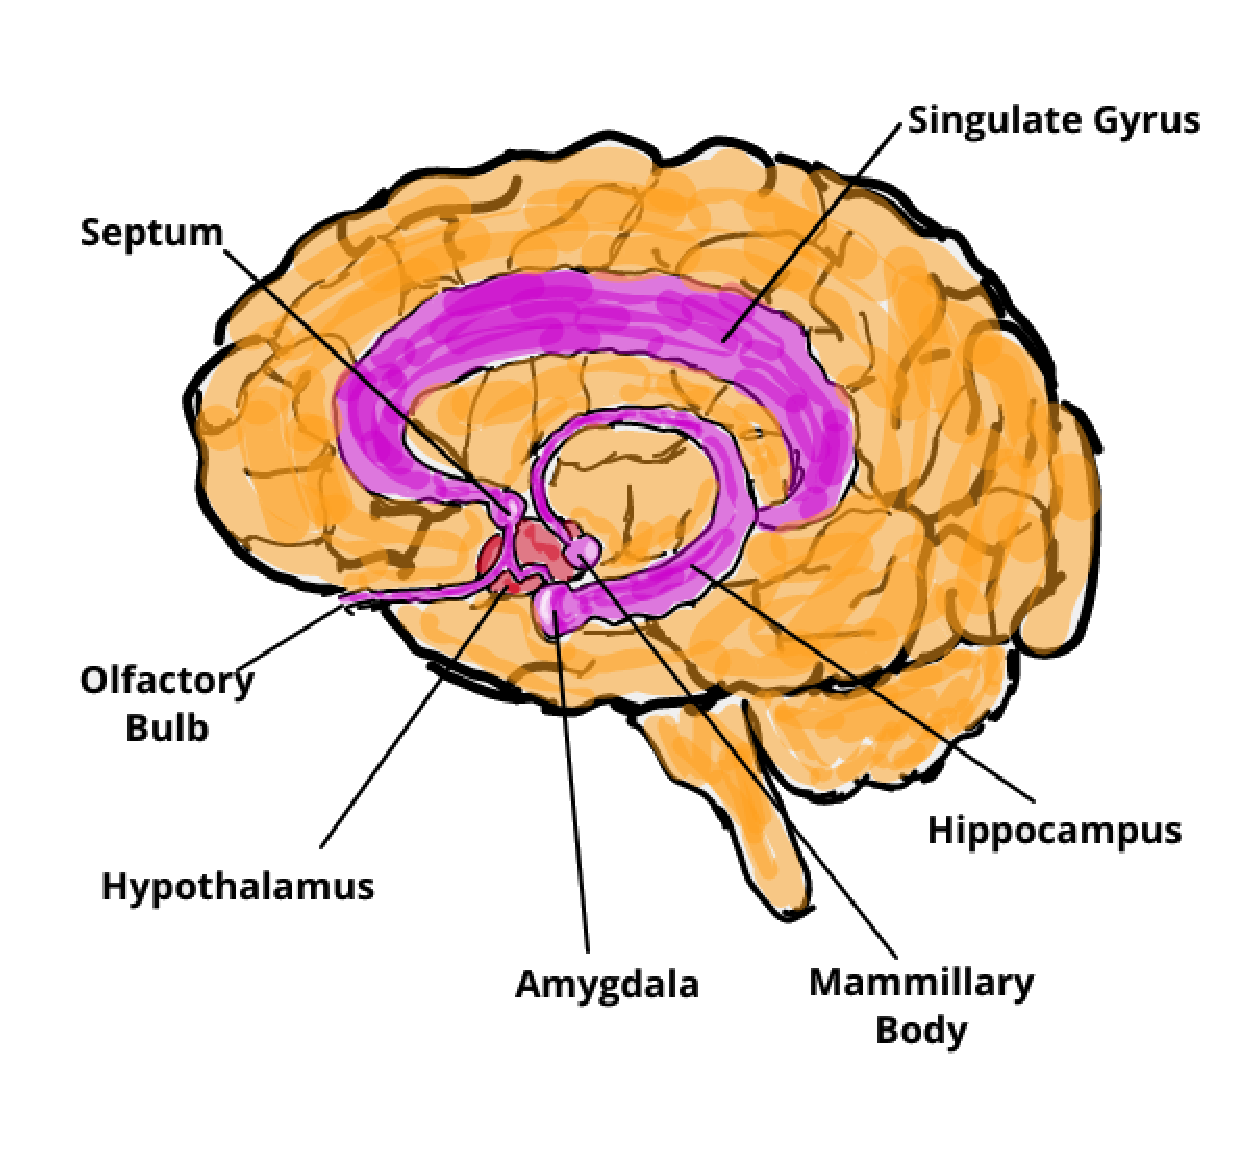
\includegraphics[width=7cm]{Limbic_System.eps}
\caption{The limbic system in the human brain.}
\end{figure}



\subsubsection{Processing in the Limbic System}

The limbic system is a {deeper lying part} of the brain, which regulates {instinctive
  reactions}\index{reaction!instinctive}, like the \emph{fight or flight} reaction in the stress situation.
Parts of this ring shaped system play a complex and important part in the {expression of drives and emotions}\index{drives}\index{emotions} and the influence of the state of the mood on the external behaviors and the memory (translated from \cite{DorlingAtlas}).
%-----------------------------------------------------------
%------------------------------------------------

The following systems get regulated in the limbic system:
\begin{enumerate}
\item {Sleep--awake state and cycle}
\item {Nutrition}
\item {Procreation}
\item {Feelings and emotions}\footnote{We distinguish between feelings and emotions. An {emotion is a reaction} to a feeling.}
\end{enumerate}


%------------------------------------------------


If one of these systems gets disturbed it will {cause a stress reaction}. Possible disturbances are sleep deprivation, eating compulsion, sexual abuse or psycho terror.
All these systems are responsible for the {alarm reaction}.

\subsubsection{Stress Regulation}


The limbic system is the {main focus of stress regulation}.
That means we watch out for a {healthy and balanced body household} in terms of\footnote{There's no such a thing as a magic pill :-) }
\begin{itemize}
\item Sleeping and waking times
\item Nutrition
\item Sexuality % xxx comment out for kids.
\item Landscape of feelings
\item Exchange of emotions
\end{itemize}



\end{document}%Good
% \mode*
% %-------------------------------------------------------------
% \subsection{Psychological Background}
% \mode<all>
% \documentclass[../Book.Stress_regulation.tex]{subfiles}
\graphicspath{{\subfix{../images/}}}
\begin{document}


In this context, two different types of strain are relevant for stress regulation.

\begin{description}
\item[Stimulus Strain]\index{strain!stimulus} is when an always recurring event makes me angry. ``My partner \textbf{always} leaves the toothbrush in the sink". 
\item[Exterior Strain:] Everybody wants to {influence and control others}. There are many examples of it in inter--human relationships. 
There's as well the self inflicted heteronomy in the visual and auditory areas (media, commercials, Animals, \ldots). 

TV influences our society and sometimes educates the kids.
\end{description}

\epigraph{We owe to TV the existence of the phenomenon, that an innumerable amount of people wake up every evening, before they go to bed.}{\textit{Robert Lembke}}


\end{document} %Good
% \mode*
% %-------------------------------------------------------------
% \subsection{Stressors}
% \mode<all>
% \documentclass[../Book.Stress_regulation.tex]{subfiles}
\graphicspath{{\subfix{../images/}}}
\begin{document}


\subsubsection{Psychological Stressors}


\begin{itemize}
\item Tendency to impatience
\item Anger
\item Engagement
\item Fear
\item Hostility
\item Dominant behavior
\item Competitiveness
\item Wrong assessment of the situation
\item To get yourself worked up in something
\item Your own time and performance pressure
\item Alarmist tendencies
\item Too high expectations for yourself
\item Disappointment
\item Imagined threats or helplessness
\item Loss of a loved one or animal 
\item Time pressure
\item Over challenged
\item Under challenged
\item Testing situation
\item Density (crowds)
\end{itemize}



\subsubsection{Social Stressors}

\begin{itemize}
\item Conflicts
\item Differences of opinions
\item Loss of relatives and close beings
\item Isolation
\item Group pressure (Mobbing)
\item Rejection by other people
\end{itemize}

\subsubsection{Chemical Stressors, Foreign substances}
\begin{itemize}
\item Nicotine
\item Alcohol
\item Drugs
\item Chemicals, ex: Deodorants, tooth paste, body lotions
\end{itemize} 
\end{document} %Long list
% \mode*

% %-----------------------------------------------------------
% \subsection{Stress regulation}
% \subsubsection{Solution oriented thinking}
% \mode<all>
% \input{salutogenesis.tex} %Good
% \mode*
% %------------------------------------------------------------
% %-----------------------------------------------------------
% \subsection{Stress and movement}
% \mode<all>
% \input{movement.tex} %Good
% \mode*
% %------------------------------------------------------------
% \section{Exercises}
% \subsection{Exercise: Sun Salutation}
% \mode<all>
% \input{Sun_Salutation.tex} %Good
% \mode*
% %---------------------------------------------------------------
% \subsection{Mindfulness and Meditation}
% \mode<all>
% \documentclass[../Book.Stress_regulation.tex]{subfiles}
\graphicspath{{\subfix{../images/}}}
\begin{document}

\setlength\epigraphwidth{.55\textwidth}

 \epigraph{I exist as I am, that is enough \\
If no other in the world be aware I sit content,\\
And if each and all be aware I sit content.\\
One world is aware, and by the far the largest to me, and that is myself,\\
And whether I come to my own today or in ten thousand or ten million years,\\
I can cheerfully take it now, or with equal cheerfulness, I can wait.}{\textit{Walt Whitman}: Leaves of Grass}
\setlength\epigraphwidth{.4\textwidth}
%includegraphics drawing myself
\section{What is Mindfulness?}

Most people, when they hear meditation, they think of {Transcendental Meditation\texttrademark} or similar relaxation practices.
In these practices you  {direct the attention to an object}, normally the perception of the inflow and outflow of the {breath or mantra} (a special sound or string of words which is repeated in your thoughts.
All other mental activity is considered {distraction}, which shouldn't be pursued.
Can induce deep states of {calmness} and {develop a steady focus}.
Also known as concentration meditation or {single focus meditation}.   

Mindfulness\index{mindfulness}, also known as {insight meditation} is another major approach to meditation.
In the beginning you use single focus attention to cultivate calmness and steadiness.
After that by {widening your object of observation}, you bring in an element of exploration.
{Thoughts or feelings}, which surface, don't get ignored, suppressed, analyzed or judged by their content.
They get consciously {observed}, as much as possible {without judgment}, how they appear as events in the field of awareness.



Ironically, this all--encompassing perception of the thoughts which appear and disappear in the mind, leads to {less getting tangled up} in them.\index{effect!thoughts, getting less tangled up}
The observer gets a {deeper insight}\index{effect!insight, deepen}\index{insight} into his reaction patterns\index{insight!reaction pattern}
to daily events and difficulties.\index{insight!difficulties}
Through the distancing from the thoughts and observing them, you can get many insights what happens {inside the mind}.\index{insight!mind}
You're able to {name the content} of the thought,\index{effect!thougths, naming} the feelings\index{effect!feeling, link to body} linked to them,
as well as the reaction to those feelings.\index{effect!feeling, reaction to it}
We get aware of our intentions\index{awareness!intentions}, fixations,\index{awareness!fixations} preferences\index{awareness!preferences},
antipathies\index{awareness!antipathies}, incoherences behind your own ideas\index{awareness!incoherence in your ideas}.
We might get insight into what drives us,\index{insight!drives} how we perceive the world\index{insight!perception of the world},
what we think\index{insight!thoughts, nature of} and who we are\index{insight!ourselves} ---
Insight into our fears\index{insight!fears} and wishes\index{insight!wishes}.

\epigraph{Music expresses that which cannot be put in words and that which cannot remain silent.}{\textit{Victor Hugo}}


{The key to practice of mindfulness} isn't so much in the object of our attention but the {quality of attention}, which we give every moment.
It's important that the attention is more like {quietly watching} and observing without taking sides, without passing judgment or instantaneously commenting the inner experiences.
It's a {pure perception}  of the momentary experience, unclouded by judgments helps us to see what is happening inside our mind {without changing}, censoring or intellectualizing it
or getting lost in never--ending thinking process.


This {observing and investigating} approach to everything which gets created in this moment is the characteristic of Mindfulness and it's at the same time the biggest difference to other forms of meditation.
The goal of mindfulness is to {be more aware and connected} with life and what happens in your body and your mind in this very moment.
If a thought or feeling is disturbing or we feel real physical {pain} we try to resist the temptation to withdraw from unpleasant experience.
Instead we try to see and accept it as clearly as possible, just because it's {present in the moment}.

Acceptance\index{acceptance} obviously doesn’t mean being passive or not caring.
On the contrary: By {accepting the moment} totally the way it is we {open ourselves} up to the experiences of life   
and we get more capable to {react appropriately} to every situation that life presents us with.
Acceptance give us a tool to navigate through the highs and lows of life. This demands of us to direct our awareness even to our\index{feelings!negative} tensions, stress, physical pain, and our mental states, like fear,
anger, frustration, insecurities, and feeling of worthlessness.
When these states emerge, {we have to meet them}, accept them and even bid them welcome.
Why? The acceptance of reality, the way it presents itself, if positive or negative, is the the {first step towards changes} of this reality and our relation to it.
 Avoiding meeting things upfront often leads to getting stuck somewhere and having difficulties to change us and to grow.


 {Don't shoot the messenger!}
Pain is only the messenger, telling you very precisely and efficiently {where something is not okay} and {what not to do} because it would make the injury worse.
It's job is to {get your attention} no matter the situation, to prevent further injury to the body. It is seriously good at it. And let's be honest, at times it is really hard to get our attention.
Listen to the message it has to deliver and {acknowledge it}, thank the pain even for the job well done and reassure it that everything will be taken care of as good as possible. 
Often that helps with the {perception of the pain}. It is still there, but it's manageable and not that needle sharp focused thing as before.

The following image might help to clarify mindfulness: {our mind is like the surface of a lake or the ocean}.
There's always {waves on the ocean}, sometimes they are big, sometimes they are small. 

Many people think the goal of meditation is to avoid the waves, so that the surface gets calm and peaceful. That's a misleading assumption.
The spirit of mindfulness is better illustrated by the picture of a 70 years old yogi with big white beard and flowing robes on a surfboard riding the waves in Hawaii. The caption says:
\begin{center}
You can't stop the waves, \\
but you can learn how to ride them.
\end{center}

\epigraph{The stars reflect as well in dirty ponds, puddles and manure run--offs}{\textit{Friedrich Georg J\"unger}, transl. from German}

\subsection{How You Can Practice Mindfulness Yourself}
\index{mindfulness!practice}
Mindfulness gets trained and practiced in two ways, both of which are essential. The first is the \emph{formal} in which we apply specific methods to help to sustain the awake and mindful state longer. The other one is the \emph{informal} practice. There we try to remember to be present in daily life and to once in a while check in if we're still being mindful. Best to imagine mindfulness as a state of being and less as a technique. At the end of the day it's the question, if and how much we're willing to be awake and present at the unfolding of our lives.

\setlength\epigraphwidth{.6\textwidth}
\epigraph{Watch your thoughts, they become words;\\
Watch your words, they become actions;\\
Watch your actions, they become habits;\\
Watch your habits, they become character;\\
Watch your character, for it becomes your destiny.}{Origin disputed.}
\setlength\epigraphwidth{.4\textwidth}

\subsection{The Formal Practice}

\index{meditation!formal} There are different forms of formal meditation, the so called \emph{body scan} (perception of the whole body, lying), the \emph{sitting meditation}, but as well different postures from hatha yoga, which get executed gently, slowly and mindfully (ex: the sun salute).
These approaches offer in multiple ways different doors into the same room.
Mindfulness of the breathing is an integral part of all of them.
First, we're looking at the sitting meditation, given that it can be practiced always and anywhere.

Each of these forms of meditation has a a focus, or a sequence of focus points, on which the the attention is directed.
Whatever focus you choose, it normally doesn't take long for the the {mind to wander off}, no matter how motivated we were to not let it happen.
Every single time this happens, we {take notice} (as nonjudgmental as possible) to where the mind has wandered, before we direct the mind {back to the object of focus}.
We might notice that we were busy with a memory, a future fantasy or a bodily perception or that we were affected of feelings of boredom, impatience or fear. Afterwards, we bring back the attention to the original object of meditation.

The aspect of bringing the attention back to a certain object resembles the one of the concentration meditation, it differs by an important element: you observe where the mind wandered. You become conscious of the changing nature of each experience and that's the core aspect of the mindfulness training.

\subsection{The Informal Practice}

The time and effort dedicated to formal practice helps to {stay present} in very the moment in daily life. 
In theory, it is very easy to be mindful during the day, but it is hard to make it into a {daily routine}. We only have to remember every moment to be present. But even tough it sounds so easy, it's hard to put it in practice.
Instead we have the habit to pass a good amount of our lives mindlessly on {autopilot}, entangled with our own thoughts, and feelings, our moods and reaction to things. Only seldom we're able to see the bigger picture.
 We are dealing with {habits} here. It is hard to break habits. The best way to go about it is to practice and {empower a new, alternate habit}.

 \epigraph{Inside of you! Inside of you is a source of goodness which never stops to bubble, as long and you don't stop digging.}{\textit{Marc Aurel}}


Mindfulness is just a {moment--to--moment awareness}, therefore every ``mundane'' task can be an opportunity to practice: eating, brushing your teeth, cleaning the dishes, walking, driving, declaring your taxes, cleaning up after your dog in the park and many other situations we're facing daily.
The wonderful advantage is that we don't need to put additional time aside.


\textbf{All what's needed is a change in consciousness. A flick of the switch from a habit--driven blind  mode of being to {awake presence}.}

In this mode, daily {life becomes practice, our meditation master and coach}.





% %---------------------------------------------------------------
% \begin{description}
% \item[Mindfulness] \index{mindfulness}
% The {informal practice} is doing this in daily life. 
% {Occurring thoughts} and feelings are noted as an outside observer.  
% The advantages of the informal practice that it needs no extra time and can seamlessly be incorporated into daily life.
% \item[Meditation] is the {formal practice} of Mindfulness, it's method--based. 
%  The {mind's focus} is on an {object}, often the breath. 
%  {Occurring thoughts} and feelings are considered a distraction and are not to be pursued.
%  \end{description}
\end{document} %Good
% \input{ANS.tex}
% \mode*

% %------------------------------------------------------------
% \section{Summary}
% \mode<all>
% \documentclass[../Book.Stress_regulation.tex]{subfiles}
\graphicspath{{\subfix{../images/}}}
\begin{document}
\section{5 Different Forms of Stress Regulation}
\index{stress regulation}
\begin{enumerate} 
\item  Daily {training of your body}\index{training} and your body awareness, to become {strong and robust}.
\item {Breathe\index{breathe} deeply} and calmly: Make every morning a gift to your body and soul, a unit of calmness and awareness, so that they beat in unison with your hearth.\\
When {thoughts} are tormenting you, observe them and write them down, or let them flow freely like a creek.
\item {Be aware}\index{awareness!body} of your body and its signals. How well do you feel getting up, at work, while eating, on the way home, in the evening by yourself?\\
Your body speaks the {language of your soul}. Be aware of what you add to your body and your soul.
\item Give the {gift of your smile}\index{smile} and laughter to the world. If you're not feeling like it, be brave and do in anyway.\\
Be aware of how the world changes.
\item Be aware of your {words}\index{awareness!words} and use them consciously: be mindful of how you speak with yourself, about how you think about and judge yourself and others.\\
Influence yourself with {positive thinking}\index{thinking!positive}. 
\end{enumerate}

\end{document}
% \mode*
% %------------------------------------------------------------

% %\section{References} % To be cleaned up, botches up article
% %\mode<all>
% %\input{Stress_References.tex}
% %\mode*

% %------------------------------------------------
% \mode
% <presentation>
% {
\begin{frame}
\Huge{\centerline{The End}}
\end{frame}}

%----------------------------------------------------------------------------------------
\mode<all>
\end{document} 
